%************************************************
\chapter{Slot Attention with Concept Supervision in CelebA-HQ}\label{ch:exp2}
%************************************************

After the literature review about Slot Attention and other Object-Centric Learning methods, where all the explanations can be found in Section --, some connections with Concept Bottleneck Models (Section --) arise naturally. Both paradigms inherently seek to decompose complex, high-dimensional visual inputs into a discrete set of interpretable variables before performing downstream reasoning. In both frameworks, the architecture forces the model to route its decision-making process through a constrained intermediate layer—whether it is a set of permutation-invariant slots representing physical entities, or a vector of semantic concepts aligned with human logic. \\
\\
Despite this shared structural philosophy, there are fundamental differences in their objectives and learning signals. Object-Centric Learning methods like Slot Attention are traditionally unsupervised, relying on spatial competition and reconstruction objectives to discover emergent, perceptual groupings. In contrast, Concept Bottleneck Models are explicitly supervised, requiring ground-truth labels to map visual features directly to predefined, high-level semantics. Furthermore, while traditional CBMs often struggle to spatially ground their concepts within specific regions of an image, Slot Attention excels at isolating localized areas but lacks the guarantee that a discovered slot will align with a human-understandable trait. \\
\\
Recognizing both the complementary strengths and the distinct differences between these approaches, this section introduces an experiment that bridges the two. By applying explicit concept supervision to a Slot Attention module, we aim to spatially ground predefined facial attributes from the CelebA-HQ dataset directly into distinct visual slots. To ensure the slots can specialize entirely on these localized semantic traits, our architecture incorporates register tokens designed to independently capture and store extra global image context. 


\begin{figure}
    \centering
    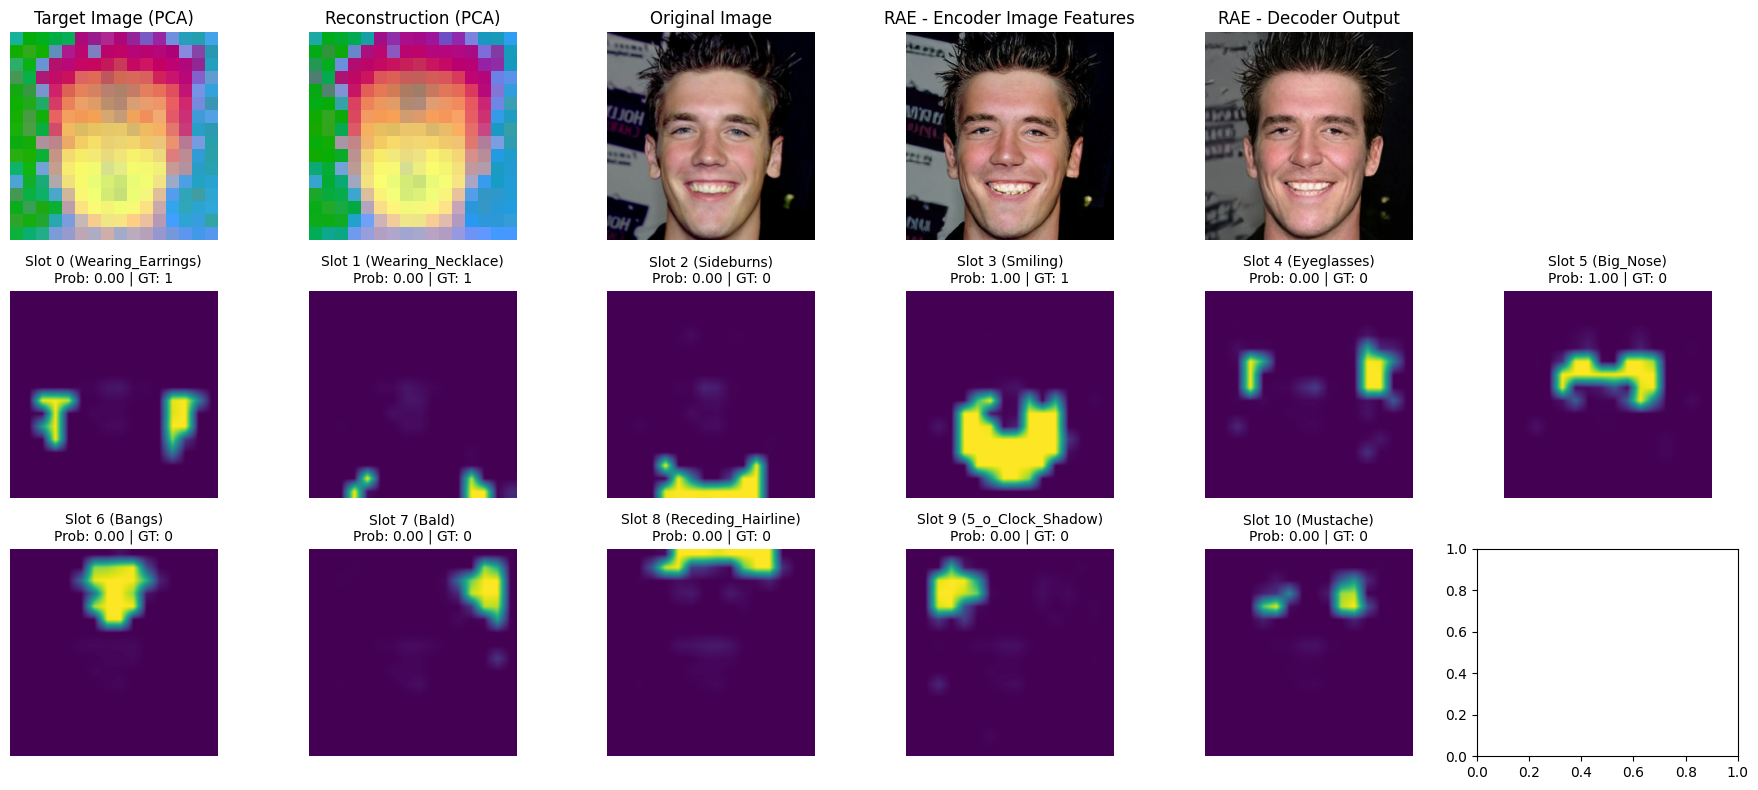
\includegraphics[width=\linewidth]{gfx/exp2/supervised_sa_1.png}
    \caption{Caption}
    \label{fig:supervised_sa_1}
\end{figure}
\begin{figure}
    \centering
    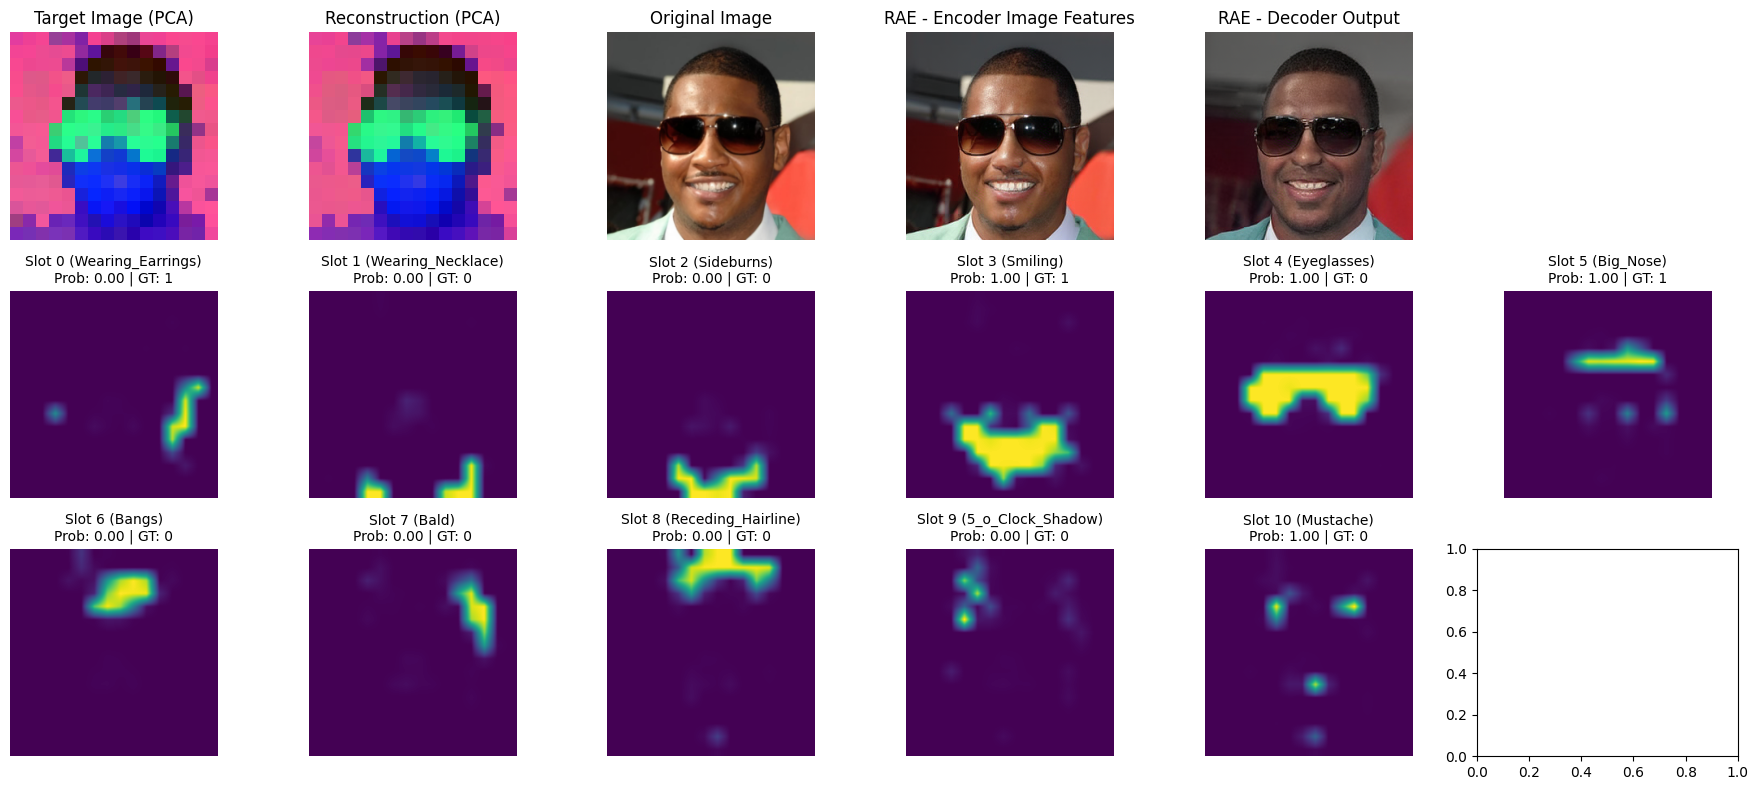
\includegraphics[width=\linewidth]{gfx/exp2/supervised_sa_2.png}
    \caption{Caption}
    \label{fig:supervised_sa_2}
\end{figure}
\begin{figure}
    \centering
    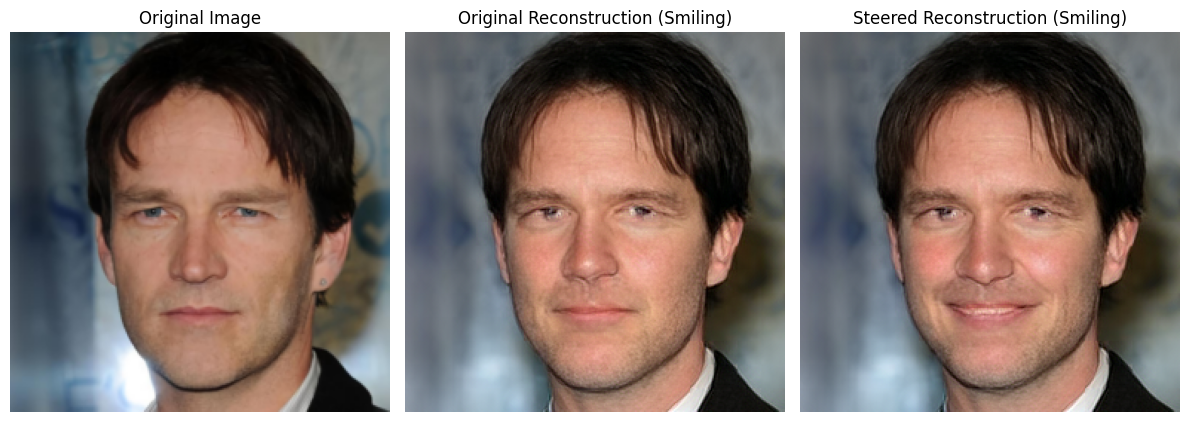
\includegraphics[width=\linewidth]{gfx/exp2/steer_smiling.png}
    \caption{Caption}
    \label{fig:steer}
\end{figure}





%*****************************************
%*****************************************
%*****************************************
%*****************************************
%*****************************************